\documentclass[12pt,a4paper]{report}
\usepackage[utf8]{inputenc}
\usepackage{amsmath}
\usepackage{amsfonts}
\usepackage{amssymb}
\bibliographystyle{acm}
\usepackage{graphicx} 
\usepackage{rotating}

\usepackage{setspace}

\renewcommand{\baselinestretch}{1.5} 

\makeatletter
\newcommand*{\toccontents}{\@starttoc{toc}}
\makeatother

\setcounter{secnumdepth}{0}
\begin{document}

\begin{center}
COSC7502 \\
Joshua Maloney - s40107464 \\
Mashhuda Glencross - Supervisor \\
\Large\textbf{Visualising Daily Solar Supply} \\
Project Thesis \\
\end{center}


\toccontents

% Abstract

\section{Abstract}

Visualising Daily Solar Supply is the journey of OpenSolar, which is a 3D visualisation of home solar power generation per day, including statistics about the percent of homes with systems, and the total estimated production per day. The visualisation emulates a virtual twin of Australian cities, and demonstrated how it could be integrated with other virtual systems such as the Internet of things. The visualisation relies on existing data sources and builds upon them by providing the daily power supply, as well as making that data discoverable for all postcodes.

\section{Introduction}

% What is it
Visualising Daily Solar Supply has produced the product OpenSolar. OpenSolar is a data processing and visualisation system. There are a number of dedicated applications as part of the system.

% What does it do
OpenSolar gathers daily data and calculates the PV power generated in the previous day.

OpenSolar can visualise solar power on a national scale, as well as zoom in to smaller, more focused geographic areas.

% Who cares about it

% Why is it so good
How much solar power is generated per day nationally? This question is hard to answer and before OpenSolar, there was no estimate of such a value to be found.

OpenSolar answers the question of how much power is being generated daily, as well as provides estimates on state, territory and postcode level.

OpenSolar increases the understandability of the data by presenting it in a visually familiar way, using 3D maps to display recognisable locations.

OpenSolar increasses ease of access to data by making the system available to users by a web browser, which is standard for modern devices including computers, tablets and phones.

OpenSolar uses existing data services to make its calculations. This leverages existing sources to create new information.

\subsection{All acronyms}

PV - photovoltaic \\
APVI - Australian Photovoltaic Intitute \\
BOM - Beareau of Meteorology \\
ABS - Australian Bureau of Statistics \\
POA - Postal Area \\
MB - Meshblock (geographic region) \\
JS - JavaScript \\


\subsubsection{Nomenclature - Geoographic terms}

\textbf{Suburb} - Throughout this thesis I will talk about suburbs, towns and localities. Although the smallest geographical region that I will consider is called a meshblock (see below), this only occurs during data processing and is not accessible to the end user. The end users will see data amalgamated into ``postcodes'', which is loosely defined as a postal region (POA). Whenever I say ``suburb'', this applies equally to suburbs, towns and postal regions.  I will generally use the word suburb for readability.

\section{Background}

\subsection{Solar Supply}

The term solar supply is fairly ambigous. Colloquially, solar power and solar energy might be considered equivalent, but in scientific terms these have distinct meanings. 

We use the definition of solar power to be the instantaneous output of a PV system. Solar power is measured in Watts (W), the units of power.

Solar energy is produced, stored and consumed over time. Solar energy depends on the solar power supply, and how long the system continues to charge at that level of power. We can calculate the solar energy by taking solar power $\times$ time. The units of solar energy are Joules (J) or often it is more convenient to work in kilowatt hours (kWh).

In the context of daily supply, it makes more sense to talk about solar energy. Solar energy is measured throughout a length of time (in our case one day) and is therefore suitable for measuring the supply provided in that time. 

The problem with visualising solar energy per day is that this data is not available anywhere. The data we have on hand turns out to be insufficient. However we can assemble enough so that we can provide a good estimate of what the daily solar power supply would look like.  This estimation ends up adding a lot of unexpected work to the project, in terms of processing and storing the new data feature, but also adds something unique that is not readily available elsewhere.

\subsection{Existing tools}

\subsection{Existing data that we want to work with}

\subsection{Technology that can support our goals}

\subsection{Final thoughts on project given background}

\section{Project Overview}

% Why Solar?
Currently there is no easy answer to the question: how much solar power is produced in Australia each day? We aim to use available data sources to estimate a reasonable number for Australia's daily solar supply. 

% What about 3D Visualisation?
The goal of the project is to apply 3D visualisation to solar data. Specifially we would like to explore daily solar supply.

% So how did you get to visualising it in a browser?
There are already some browser based solutions for exporing climate data and PV statistics. This project aims to emphasis solar supply on a much more local scale, by visualising suburb-sized localities. The scale of solar supply can be shown for a neighbourhood, and also these are collected together to show total supply for each state as well as the national solar supply. 

Browser support is important to remain accessible to a reasonable amount of devices. Because the technologies that we are using are standardised, we can expect compatablity with any device currently capable of running a web browser. 

As a developer, these standards offer good performance as well as powerful 3D graphics capabilities.

% What source data did you know you needed?
The final structure of the application is a result of the format of the data, in order to make the processing possible.

Source data from APVI was already divided into postcodes.

Maps and elevation are available as PNG.

% What source data did you find out you also needed?
There were also some extra data sources that we needed to find and manage, because the scope of the project had expanded from the initial proposal and the data sources we knew about no longer were able to fill the gaps. Some extra data sources were necessary to be added in to the project.

Because we had PV system capacity by postcode, theoretically we could calculate the supplied power per day if we knew how sunny it was. Some research showed that other climate tools were tracking a quantity known as solar irradiance. Solar irradiance measures how much energy from the sun falls on an area of $1 \text{m}^2$. Source data summarising the daily solar irradiance is available from BOM. The data covers all of Australia with a lat-lon grid. 

The summary is provided as a .Z file, this was unexpected and not able to be processed without tools. The tools then required an environment to run, and the envoronment needed to be hosted such that it could execute on a daily schedule. The simple need to unzip a file had extensive imacts on the very design of this application.

% Making preperation to develop the secret formula

% Coding process for the visualisation

% Container process for the estimation

% Centralising by Github

\section{Project Design - Initial Planning}

\section{Project Design - Replanning and Focus Features}

\section{Project Design - Final Implementation}

% Kind of building and elaborating on the background

% Building the container
\subsection{Designing the processing phase}
The BOM data is provided in a .Z file, and it turned out the only practical way to decompress .Z files is with gzip. Using gzip would require a Linux command line. So a container was a practical solution to this small detail.

Zip in Python didn't work. 

A Linux was needed because I had to invoke gz to actually read the file data. 

A container allowed Python sctipting as well as accessing shell commands. I could then unzip the file, do some data processing, then create a processed data file set which could be uploaded to the visualisation.


\subsection{Designing the visualisation}

Initially I wanted to have a site that could access data from an external service, like one of many available cloud platforms. This seemed convenient because cloud platforms could also execute some Python scripts and do the processing and data hosting all in the same place. As well as the processing not being sufficient, there would be problems with cross site domain access, and it was not efficient as a simple solution that could just access the files that were needed.

A more suitable approach was to use a visualisation as a static website using the existing framework provided by github pages. The data files themselves can be updated daily by the processing app, which does so with its own github account.

The static files are then read directly by the website.

\subsection{Explain the parts of the project}

There are parts of the data that need to be processed together. For example, getting the name of a postcode region is not so simple, even questions about what state it's in can be ambiguous. We take the source data and process it in a way that makes sense for us. We consider postcode areas, so we would like to know the location of where a postcode is, and the name of the region.

A processing phase will calculate that and provide a table that we will use in the visualisation.

\includegraphics[scale=0.42]{file_process_1.eps}

\subsection{Explain limitations of why it was caused to be that way}

\section{Project Parts and Subprojects?}

\subsection{Project Tools and Work Environment}

Most of the project implementation involves writing code in some way. The text editors used were Atom, SublimeText, Visual Studio Code. Atom is free and open source, SublimeText is trial that requires full version to be paid for, Visual Studio Code is free.

The code then needs to be compiled to a release format. Emscripten is used to generate WASM and JS bindings. 

All tools are used on a Linux Ubuntu work environment.

\subsection{What is a postcode anyway?}

Postcodes are generally dictated by Australia Post, there is not a specific boundary to any postal code.

A postcode refers to what the ABS would call a postal area (POA). A POA is a collection of meshblocks that are assigned the same postcode. 

So what is a meshblock?

A meshblock (mb) is a geographical region which is provided with a uniquely identifying code. A meshblock is the smallest region considered my the ABS. Meshblocks vary in the size of the geographical area, but are divided in such a way that approximately 50 residents live in any given meshblock. This designation is small enough to be useful for fine-grained geographical systems, but large enough to be considered anonymising. 

We can gather data from the ABS that identifies all meshblocks in Australia, together with the geographical area, postcode and locality (town or suburb) name.

This data is essential for creating a user interface to our application. We must allow the user to search for a location by name, and provide a result. We therefore need the postcode of that suburb name, as well as the location of the suburb.

The ABS provides CSV data as well as a GPKG. To access the data in a GPKG, we need to use specialised software. I have chosen to use GDAL to access the data and use a Python script to process everything that I need. 

The goal of the script is to scan through every meshblock in the GPKG file, and figure out the geographic location. This is simplified by taking the AABB only. The final goal of this process is to have a centre point which coresponds to each suburb.

After this processing phase, I should be able to search for a suburb by name, and tell you the postcode as well as a (lon, lat) pair giving the approximate centre point.

This will allow the user to type the name of the suburb, or it's postcode, and have the application zoom into that area with some accuracy. 

\subsection{Building the Postcode Data Sets}

\subsubsection{visualisation data from the GPKG}

One important thing is to know where a POA is.

We can find this by exploring the shapes in the GPKG. The extents of each feature give a simple way to keep track of the general area where you would find that suburb.

This allows us to zoom in to any location by postcode.

But what if we want to find a location by name?

The solution to this problem is to generate a map of names to postcodes. We can also create this map from the GPKG. Although we have to be careful because some postcodes have more than one name, for example 4000 is the postcode of Spring Hill and Brisbane City. We can use this name:postcode map to find out the postcode of an area by matching a partial string to the names of all suburbs.

From this system we can go from a name or partial name, to a key matching string which gives a postcode and then the longitute and latitude of the POA.

\subsubsection{visualisation data for solar}

By having the postcode and being able to expore it easily allows further visualisation of the solar data.

We can calculate daily solar supply because the installation data is clustered by each postcode.

Using the postcode data and geographic location, we can mix with the latest daily solar irradiance map to find the expected supply of solar energy. The location can be read from the processing of shapes that we did in the previous step.

The resultant data is tabulated into postcodes and supply amounts, then it is uploaded to the file host, and the visualisation can read the data from static files in real time.
 
\subsubsection{processing the solar data}

\subsubsection{Co-ordinate systems}

Generally all of the geographic data is supplied using a pair of co-ridinates, latitude and longitude. For visualisation purposes, we want to project these points into 3D space.

The web mapping format uses the Mercator projection. 

We project lat-lon pairs into 3D space using this projection and an elevation parameter.

Geographic space -> 3d (ecef) space 
Earth space -> local space 
3D space -> screen space 

Mapping tiles to geometry and focusing on a geographic feature.

Converting screen co-ordinates back to geographic co-ordinates.

\subsubsection{Building terrain for the visualisation}

Terrain is an important aspect of the virtual world. The map will show natural features on the ground and elevation differences that are important in identifying locations that are unique.

Raster data sources are taken at real-time, when a location is chosen to be visualised. 

Elevations maps are turned into mesh geometry and tile maps are used to texture the geometry.

The terrain is created using a tile system. The tile or tiles to be used will be determined by the geographic bounds of the postcode region. The postcode bounds are used to find the max and min tile numbers in longitude and latitude directions. Each tile is then downloaded and converted into 3D mesh.

This process requires that the visualisation has access to the geographic data associated with each postcode. 

%https://en.wikipedia.org/wiki/Tiled_web_map

Tile Map Service: (0 to $2^{zoom}-1$, $2^{zoom}-1$ to 0) for the range (-180, +85.0511) - (+180, -85.0511). (That is, the same as the previous with the Y value flipped.)

\section{Discussion}

\subsection{Usefulness and exploration of the data}
\subsubsection{Database vs visualisation}


\subsection{PV networks}
\subsubsection{IoT integration}
\subsubsection{Blockchain PV trading}
Power Ledger is one system using a blockchain for trading the supply of PV systems supply. The advantages of using a blockchain system include transparacy and a secure and permanant record.
\subsubsection{Smart Contracts}
As a platform, Etherium was built to create and enact smart contracts. The concept of smart contracts is a programmable script that can interact with the blockchain, but costs money to store and run. 

Smart contracts in Etherium are designed to compile into WASM binary code, or a subset called EWASM.
\subsubsection{WASM in Visualisation}
Our visualisation is already equipped to run with WASM binary code, so therefore there is the capacity to integrate with Etherium and Power Ledger. In this case it would further increase the scope of the visualisation by providing real time supply data and consumtion of systems locally in a network.

%\bibliography{bb}

\end{document}